\section{Implementierung der Delivery Queue} \label{dlq}

Die Delivery Queue enthält alle Nachrichten, die an den Leser ausgeliefert werden dürfen. Sie hat einen begrenzten Speicher zur Verfügung, welcher nicht überschritten werden darf. Dieser wird bei Initialisierung der Queue übergeben und innerhalb der Queue gespeichert. Die eigentliche Delivery Queue wird als First In - First Out Liste implementiert. Die Nachricht die als erstes eingefügt wurde, verlässt also als erstes auch wieder die Liste (siehe Abbildung \ref{fig:fifo}).

\begin{figure}[htbp]
\begin{center}
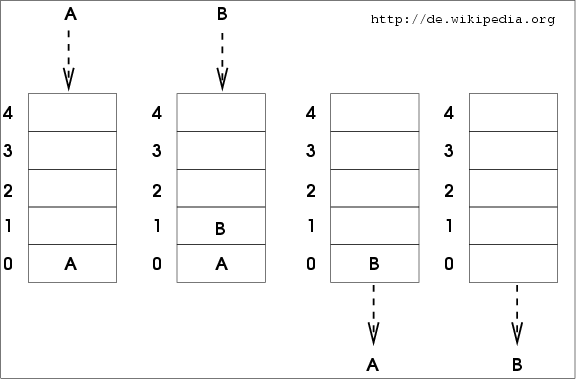
\includegraphics[scale=0.4]{Latex/Bilder/FIFO_PEPS.png}
\caption[First In First Out]{FIFO\footnotemark}\label{fig:fifo}
\end{center}
\end{figure}
\footnotetext{\url{https://de.wikipedia.org/wiki/First_In_–_First_Out}}

Dafür werden nun also die neuen Elemente immer an die Liste angehängt, so dass die Nachricht mit der kleinsten Nummer immer am letzter Stelle eingefügt wird. Hierfür bietet sich in Erlang das Anfügen an. 

\begin{lstlisting}
NewDLQ = OldDLQ ++ [NewMessage]
\end{lstlisting}

Da in dieser Funktion zwei Listen zu einer kombiniert werden, muss das zweite Element als Liste übergeben werden. Es ist als Form NewMessage = [NNr, Msg, TSclientout, TShbqin, TSdlqin] zwar schon eine Liste, aber da die Nachricht als ein Element eingefügt werden soll, muss es als Liste mit nur einem Element angefügt werden werden. 
Die Liste wird aufsteigend sortiert, da theoretisch genauso viele Elemente in die Liste eingefügt, wie auch wieder aus der Queue gelöscht werden. 

Ein Problem bei der Delivery Queue stellt die vorgegebene maximale Größe dar. Da diese nicht im Speicherplatz reserviert werden kann (keine In-Place Lösungen in Erlang), wie zum Beispiel über ein malloc in C oder über ein Attribut wie in Java, muss die Größe hier im Prozess der Queue oder direkt in der Queue gespeichert werden.
Die erste Möglichkeit zur Speicherung der Größe bietet aber viele Fehlerquellen. Die Implementierung würde wie folgt aussehen:
\begin{lstlisting}
spawn(fun() -> loop(Size, Datei, 0) end).

loop(MaxSize, Datei, ActSize) -> 
    receive 
        {From, getVariables} -> 
            From ! {reply, {MaxSize, Datei, ActSize}}
            loop(MaxSize, Datei, ActSize);
        {From, setVariables, {NewMaxSize, NewDatei, NewActSize}}
            From ! {reply, variablesSet}
            loop(NewMaxSize, NewDatei, NewActSize)
    end.
\end{lstlisting}

Über die Schnittstelle \{self(), getVariables\} und \{self(), setVariables, \{NewMaxSize, NewDatei, NewActSize\}\} können nun sowohl von der Holdback Queue, als auch von der Delivery Queue aus das Limit der Delivery Queue, die aktuelle Größe und die logging-Datei gelesen und geschrieben werden. Die Delivery Queue wäre somit eine zum Teil entfernte abstrakte Datenstruktur. 
Ein Problem, welches nach der Implementierung entstanden ist, war das sehr aufwändige Debuggen von Fehlern oder Aufrufen innerhalb der Delivery Queue. 

Eine einfachere Lösung wäre das Speichern der Variablen innerhalb der Queue. 
Diese neue Queue hat die Struktur eines Tupels mit drei Elementen, welche zum einen die maximale Größe und die aktuelle Größe sind und zum anderen die eigentliche Queue in Form einer Liste - also DLQ = \{MaxSize, ActSize, [Msg1, Msg2, ...]\}. So werden mögliche Fehler, welche durch Nebenläufigkeiten entstehen können, eliminiert. \\
Im Folgenden wird mit der zweiten Lösung, also der Speicherung der Elemente innerhalb der Delivery Queue als Tupel, gearbeitet.

\subsection{Operationen}

\subsubsection{initDLQ}

In der Initalisierungfunktion der Delivery Queue wird die Queue erzeugt. Die Funktion hat den Aufruf initHBQ und bekommt die maximale Größe und die logging-Datei mit übergeben. 
Nach erfolgreicher Initialisierung wird die Initilialsierungsgröße der Delivery Queue geloggt und ein Tupel mit den Elementen MaxSize, ActSize und der eigentlichen Queue zurückgegeben.

\subsubsection{delDLQ}

Da die Delivery Queue in dieser Implementierung nicht als entfernte abstrakte Datenstruktur umgesetzt wurde, muss auch dementsprechend kein Prozess beendet werden. Die Funktion gibt also beim Aufruf nur ein 'ok' zurück.

\subsubsection{expectedNr}

Diese Funktion liefert die Nachrichten Nummer die als nächstes in der Delivery Queue gespeichert werden kann. Da die kleinste Nummer von dem Leser Client benötigt wird und außerdem keine Duplikate vorkommen sollten, wird in der Delivery Queue die größte Nummer gesucht und diese um eins erhöht. Die größte Nummer ist stets das letzte Element der Delivery Queue. Es wird also rekursiv eine Teilliste der Queue aufgerufen und das erste Element dieser gespeichert, bis die Teilliste leer ist (siehe getLastElem/1). Auf das zuletzt gespeicherte Element wird eine 1 addiert und das Ergebnis ist die erwartete Nummer. 
\begin{lstlisting} 
getLastElem([[NNr, _Msg, _TSclientout, _TShbqin, _TSdlqin]|[]]) -> NNr;
getLastElem([_Head|Tail]) -> getLastElem(Tail).
\end{lstlisting}

\subsubsection{push2DLQ}

Diese Funktion wird von der Holdback Queue aufgerufen, wenn diese eine bestimmte Größe erreicht hat und Elemente an die Delivery Queue übergibt. Die zugehörige Schnittstelle der Holdback Queue ist \{self(), \{request, pushHBQ, Msg\}\}.

Die Funktion push2DLQ speichert die übergebene Nachricht in der Delivery Queue. Da die Queue bereits sortiert ist und das letzte Element in der Queue das Größte ist, kann das neue Element einfach an die Liste angefügt werden. Zusätzlich wird ein Zeitstempel angefügt, welcher über eine von Erlang bereitgestellte Funktion erfasst wird. 
Bei jedem Funktionsaufruf wird außerdem die maximale Größe mit der aktuellen Größe verglichen. Wenn die Delivery Queue die maximale Größe erreicht hat, dann wird beim Einfügen eines neuen Elements das Älteste gelöscht. Dies kann in Erlang sehr effizient umgesetzt werden. Durch die Aufteilung der Liste in Startelement und Restliste kann zum Löschen des ersten Elements einfach mit der Restliste weitergearbeitet werden. 
% obereren Satz schonmal verwendet?

\begin{figure}[htbp]
\begin{center}
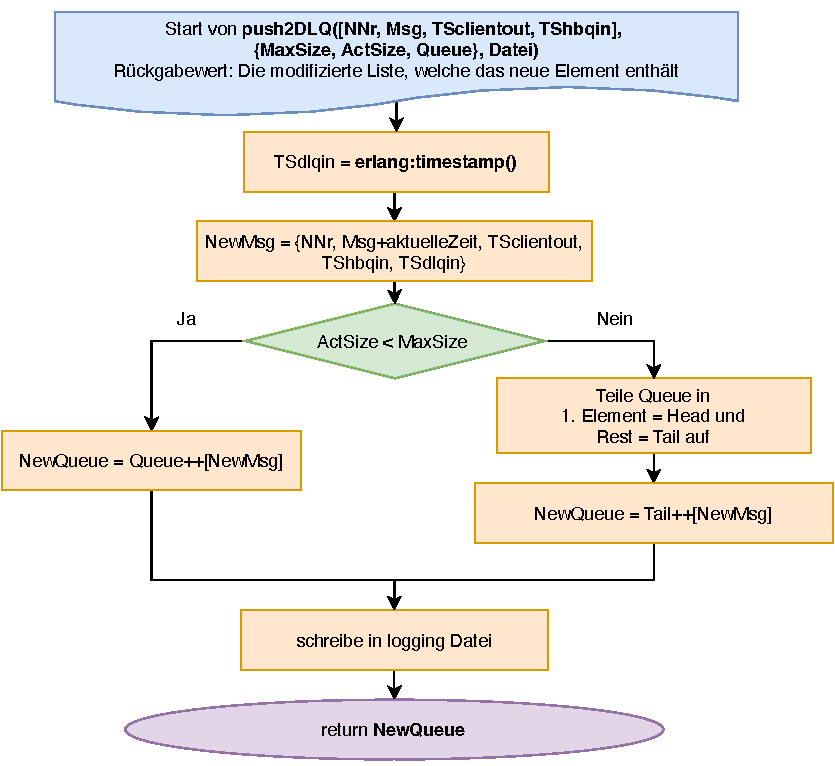
\includegraphics[scale=0.65]{Latex/Bilder/push2DLQ.pdf}
\caption{pushDLQ}\label{fig:pushDLQ}
\end{center}
\end{figure}

\subsubsection{deliverMSG}

Diese Funktion sendet die im Parameter übergebene Nachrichtennummer an die übergebene ProzessID des Clients. Dafür wird durch die Elemente der Delivery Queue gelaufen, bis das Element entweder gefunden wurde oder das übergebene Element größer ist. 

\begin{lstlisting}
getMSGAtMSGNr(_MSGNr, []) -> [-1,nokb,0,0,0];
getMSGAtMSGNr(MSGNr, [[NNr, Msg, TSclientout, TShbqin, TSdlqin]|_Tail]) when MSGNr =< NNr-> 
    [NNr, Msg, TSclientout, TShbqin, TSdlqin];
getMSGAtMSGNr(MSGNr, [_Head|Tail]) -> getMSGAtMSGNr(MSGNr, Tail).
\end{lstlisting}

In obiger Funktion ist noch einmal das rekursive Durchlaufen der Liste gezeigt. Der Funktion wird eine Liste übergeben, in diesem Falle die Delivery Queue und dann wird von dieser Liste so oft das erste Element abgeschnitten, bis eine der beiden Abbruchbedingungen eintreffen. Anhand von Pattern Matching kann dann effizient verglichen werden, ob die Liste leer ist oder ob die erste Nachricht der übergebenen Liste größer gleich der gesuchten Nachrichtennummer ist.
Gelöscht werden die Elemente aus der Delivery Queue allerdings erst, sobald diese ihre maximale Größe erreicht hat und somit durch die Funktion push2HBQ verkleinert wird. 
Das eigentliche Senden der Nachricht an den Clienten findet innerhalb der Delivery Queue statt. \\Der Aufruf hat den Aufbau:
ClientPID ! \{reply,SendMessage,Terminated\}

Um den gesamten Prozess terminieren zu können, wird der Delivery Queue von der Holdback Queue mitgeteilt ob diese noch Elemente enthält. Wenn das nicht mehr der Fall ist wird die Nachricht [-1,nkob,0,0,0] mit einem weiteren Parameter true übergeben, welcher signalisiert, dass der Prozess beendet werden soll. 

\subsubsection{listDLQ}

Die Funktion gibt eine Liste mit den Nummern der in der Delivery Queue enthaltenden Nachrichten zurück. Die Nummern werden nach aufsteigender Größe sortiert sein, da am Kopf der Queue angefangen wird. Somit ist also auch die Reihenfolge der Liste eingehalten. 

\subsubsection{lengthDLQ}

Diese Funktion gibt die Anzahl der in der Delivery Queue enthaltenden Nachrichten zurück. Dafür kann die im Tupel der Delivery Queue enthaltende Variable ActSize zurückgegeben werden. 